\section{固有振動モードの変動に関する方程式}

\begin{figure}[ht]
	\begin{center}
		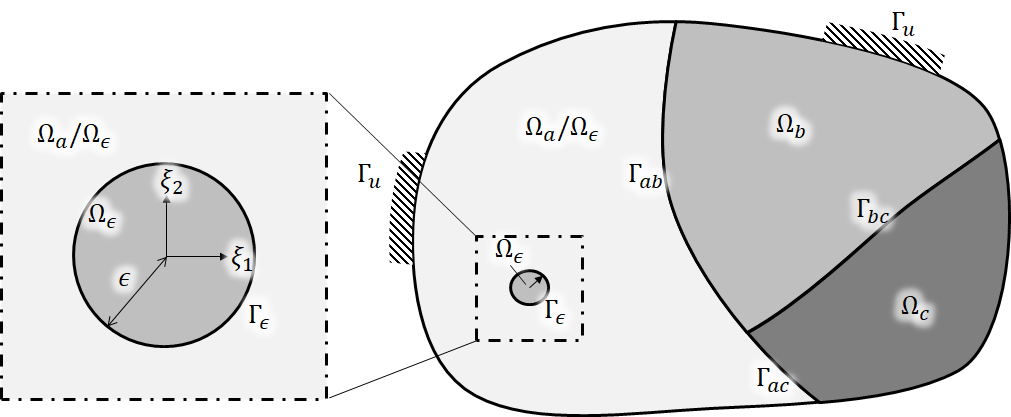
\includegraphics[width=13cm]{./figures/TD.png}
		\caption{Topological derivative}
		\label{fig:TD}
	\end{center}
\end{figure}

固有振動モードの変動$\hat{\bm{u}}(\bm{\xi})$に関する支配方程式は以下のようになる.
\begin{align}
&C_{ijkl}^{b} \hat{u}^{(-)}_{k,lj}(\bm{\xi})
+\epsilon^2\{(\lambda+\hat{\lambda})\rho^{b} \hat{u}_{i}^{(-)}(\bm{\xi})\}=0&\text{in}\hspace{0.3cm}\Omega_{\epsilon}
\label{eq:GovDisturIn}
\\
&C_{ijkl}^{a}\hat{u}^{(+)}_{k,lj}(\bm{\xi})
+\epsilon^2\Bigl \{\lambda\rho^{a} \hat{u}_{i}^{(+)}(\bm{\xi})
+\hat{\lambda}\rho^{a} \bigl(u_{i}^{}(\bm{x})+\hat{u}_{i}^{(+)}(\bm{\xi}) \bigr) \Bigr \}=0
&\text{in}\hspace{0.3cm}\Omega\backslash\Omega_{\epsilon}
\label{eq:GovDisturOut}
\\
&\hat{u}_{i}^{(-)}(\bm{\xi})-\hat{u}_{i}^{(+)}(\bm{\xi})=u_{i}(\bm{x})=u_{i}(\bm{x_0})+\epsilon \xi_j u_{i,j}(\bm{x_0})+O(\epsilon^2) &\text{on}\hspace{0.3cm}\Gamma_{\epsilon}
\label{eq:GovDisturUBC}
\\
&C_{ijkl}^{b}\hat{u}_{k,l}^{(-)}(\bm{\xi})n_{j}^{(-)}
-C_{ijkl}^{a}\hat{u}_{k,l}^{(+)}(\bm{\xi})n_{j}^{(-)}
=\epsilon C_{ijkl}^{a}u_{k,l}(\bm{x_0})n_{j}^{(-)}+O(\epsilon^2) &\text{on}\hspace{0.3cm}\Gamma_{\epsilon}
\label{eq:GovDisturSBC}
\\
&\sum_{p=1}^{n}\int_{\Omega_p}\rho^{p}(2u_{i}\hat{u}_{i}^{(+)}+\hat{u}_{i}^{(+)}\hat{u}_{i}^{(+)}) d\Omega
+\int_{\Omega_{\epsilon}}\{\rho^{b}\hat{u}_{i}^{(-)}\hat{u}_{i}^{(-)}-\rho^{a}u_{i}u_{i}\} d\Omega=0
\label{eq:GovDisturNorm}
\\
&\hat{u}_{i}^{(+)}(\bm{\xi})\rightarrow 0 \hspace{0.3cm} (|\bm{\xi}|\rightarrow \infty)
\label{eq:GovDisturInftyBC}
\end{align}

$\epsilon$の0次の項を整理すると
\begin{align}
&C_{ijkl}^{b} \hat{u}^{(I-)}_{k,lj}(\bm{\xi})=0&\text{in}\hspace{0.3cm}\Omega_{\epsilon}
\label{eq:GovDisturIn1}
\\
&C_{ijkl}^{a} \hat{u}^{(I+)}_{k,lj}(\bm{\xi})=0&\text{in}\hspace{0.3cm}\Omega\backslash\Omega_{\epsilon}
\label{eq:GovDisturOut1}
\\
&\hat{u}_{i}^{(I-)}(\bm{\xi})-\hat{u}_{i}^{(I+)}(\bm{\xi})=u_{i}(\bm{x_0}) &\text{on}\hspace{0.3cm}\Gamma_{\epsilon}
\label{eq:GovDisturUBC1}
\\
&C_{ijkl}^{b}\hat{u}_{k,l}^{(I-)}(\bm{\xi})n_{j}^{(-)}
-C_{ijkl}^{a}\hat{u}_{k,l}^{(I+)}(\bm{\xi})n_{j}^{(-)}=0 &\text{on}\hspace{0.3cm}\Gamma_{\epsilon}
\label{eq:GovDisturSBC1}
\\
&\hat{u}_{i}^{(I+)}(\bm{\xi})\rightarrow 0 \hspace{0.3cm} (|\bm{\xi}|\rightarrow \infty)
\label{eq:GovDisturInftyBC1}
\end{align}

$\epsilon$の1次の項を整理すると
\begin{align}
&C_{ijkl}^{b} \hat{u}^{(I\hspace{-.15em}I-)}_{k,lj}(\bm{\xi})=0
&\text{in}\hspace{0.3cm}\Omega_{\epsilon}
\label{eq:GovDisturIn2}
\\
&C_{ijkl}^{a} \hat{u}^{(I\hspace{-.15em}I+)}_{k,lj}(\bm{\xi})=0
&\text{in}\hspace{0.3cm}\Omega\backslash\Omega_{\epsilon}
\label{eq:GovDisturOut2}
\\
&\hat{u}_{i}^{(I\hspace{-.15em}I-)}(\bm{\xi})
-\hat{u}_{i}^{(I\hspace{-.15em}I+)}(\bm{\xi})= \xi_j u_{i,j}(\bm{x_0})=u_{i}^{(I\hspace{-.15em}I)} &\text{on}\hspace{0.3cm}\Gamma_{\epsilon}
\label{eq:GovDisturUBC2}
\\
&C_{ijkl}^{b}\hat{u}_{k,l}^{(I\hspace{-.15em}I-)}(\bm{\xi})n_{j}^{(-)}
-C_{ijkl}^{a}\hat{u}_{k,l}^{(I\hspace{-.15em}I+)}(\bm{\xi})n_{j}^{(-)}
=C_{ijkl}^{a} u_{k,l}^{}(\bm{x_0})n_{j}^{(-)}=t_{i}^{(I\hspace{-.15em}I)} &\text{on}\hspace{0.3cm}\Gamma_{\epsilon}
\label{eq:GovDisturSBC2}
\\
&\hat{u}_{i}^{(I\hspace{-.15em}I+)}(\bm{\xi})\rightarrow 0 \hspace{0.3cm} (|\bm{\xi}|\rightarrow \infty)
\label{eq:GovDisturInftyBC2}
\end{align}
以上から,$\hat{\bm{u}}^{(I-)}$,$\hat{\bm{u}}^{(I+)}$,$\hat{\bm{u}}^{(I\hspace{-.15em}I-)}$,$\hat{\bm{u}}^{(I\hspace{-.15em}I+)}$は,それぞれ平衡方程式に従うことが分かる.

\newpage
